\documentclass[sn-basic,NameDate]{sn-jnl}\usepackage[]{graphicx}\usepackage[]{xcolor}
% maxwidth is the original width if it is less than linewidth
% otherwise use linewidth (to make sure the graphics do not exceed the margin)
\makeatletter
\def\maxwidth{ %
  \ifdim\Gin@nat@width>\linewidth
    \linewidth
  \else
    \Gin@nat@width
  \fi
}
\makeatother

\definecolor{fgcolor}{rgb}{0.345, 0.345, 0.345}
\newcommand{\hlnum}[1]{\textcolor[rgb]{0.686,0.059,0.569}{#1}}%
\newcommand{\hlstr}[1]{\textcolor[rgb]{0.192,0.494,0.8}{#1}}%
\newcommand{\hlcom}[1]{\textcolor[rgb]{0.678,0.584,0.686}{\textit{#1}}}%
\newcommand{\hlopt}[1]{\textcolor[rgb]{0,0,0}{#1}}%
\newcommand{\hlstd}[1]{\textcolor[rgb]{0.345,0.345,0.345}{#1}}%
\newcommand{\hlkwa}[1]{\textcolor[rgb]{0.161,0.373,0.58}{\textbf{#1}}}%
\newcommand{\hlkwb}[1]{\textcolor[rgb]{0.69,0.353,0.396}{#1}}%
\newcommand{\hlkwc}[1]{\textcolor[rgb]{0.333,0.667,0.333}{#1}}%
\newcommand{\hlkwd}[1]{\textcolor[rgb]{0.737,0.353,0.396}{\textbf{#1}}}%
\let\hlipl\hlkwb

\usepackage{framed}
\makeatletter
\newenvironment{kframe}{%
 \def\at@end@of@kframe{}%
 \ifinner\ifhmode%
  \def\at@end@of@kframe{\end{minipage}}%
  \begin{minipage}{\columnwidth}%
 \fi\fi%
 \def\FrameCommand##1{\hskip\@totalleftmargin \hskip-\fboxsep
 \colorbox{shadecolor}{##1}\hskip-\fboxsep
     % There is no \\@totalrightmargin, so:
     \hskip-\linewidth \hskip-\@totalleftmargin \hskip\columnwidth}%
 \MakeFramed {\advance\hsize-\width
   \@totalleftmargin\z@ \linewidth\hsize
   \@setminipage}}%
 {\par\unskip\endMakeFramed%
 \at@end@of@kframe}
\makeatother

\definecolor{shadecolor}{rgb}{.97, .97, .97}
\definecolor{messagecolor}{rgb}{0, 0, 0}
\definecolor{warningcolor}{rgb}{1, 0, 1}
\definecolor{errorcolor}{rgb}{1, 0, 0}
\newenvironment{knitrout}{}{} % an empty environment to be redefined in TeX

\usepackage{alltt}

\usepackage{lmodern}
\usepackage{amsmath,amssymb,amsfonts}
\usepackage{manyfoot}
\usepackage{booktabs}

\usepackage[document]{ragged2e}
\usepackage{parskip}

\hyphenpenalty=10000
\hbadness=10000

\setlength{\tabcolsep}{4pt}

\usepackage{setspace}
\onehalfspacing

\bibpunct{(}{)}{;}{a}{}{,}

\usepackage{lineno}
\linenumbers

%\newcommand{\okina}{`}
\DeclareRobustCommand{\okina}{%
  \raisebox{\dimexpr\fontcharht\font`A-\height}{%
    \scalebox{0.8}{`}%
  }%
}

\newcommand{\Hawaii}{Hawai\okina i}
\newcommand{\Oahu}{O\okina ahu}
\newcommand{\Milolii}{Miloli\okina i}

\newcommand{\orig}[1]{{\color{red}(#1)}}
\newcommand{\xorig}[1]{{\color{olive}(#1)}}

\title{Four decades of green turtle (\emph{Chelonia mydas}) strandings on \Hawaii\ Island (1983--2022): Causes and trends
}
\author[1]{\fnm{Skylar} \sur{Dentlinger}\textsuperscript{\dag}}

\author*[1]{\fnm{Karla J.} \sur{McDermid}}\email{mcdermid@hawaii.edu, orcid.org/0000-0002-7663-6545}
%\equalcont{These authors contributed equally to this work.}

\author[2]{\fnm{Grady} \sur{Weyenberg}}\email{gradysw@hawaii.edu, orcid.org/0000-0001-6128-1772}
%\equalcont{These authors contributed equally to this work.}

\author[3]{\fnm{Laura M. R.} \sur{Jim}}
\author[3]{\fnm{Marc R.} \sur{Rice}}\email{mrice@hpa.edu, orcid.org/0009-0008-5951-0749}
\author[4]{\fnm{George H.} \sur{Balazs}}

\affil[1]{\orgdiv{Department of Marine Science}, \orgname{University of \Hawaii\ at Hilo},
\orgaddress{\city{Hilo}, \state{Hawaii}, \postcode{96720}, \country{USA}}}

\affil[2]{\orgdiv{Department of Mathematics}, \orgname{University of \Hawaii\ at Hilo}, 
\orgaddress{\city{Hilo}, \state{Hawaii}, \postcode{96720}, \country{USA}}}

\affil[3]{\orgdiv{Sea Turtle Research Program}, \orgname{\Hawaii\ Preparatory Academy}, 
\orgaddress{\city{Kamuela}, \state{Hawaii}, \postcode{96743}, \country{USA}}}

\affil[4]{\orgname{Golden Honu Services of Oceania}, 
\orgaddress{\city{Honolulu}, \state{Hawaii}, \country{USA}}}

\presentaddress{\textsuperscript{\dag} \orgdiv{Rosenstiel School of Marine and Atmospheric Science}, \orgname{University of Miami}, \orgaddress{\city{Miami}, \state{Florida}, \postcode{33149}, \country{USA}}}


\miscnote{Note to publisher: The Hawaiian letter \okina okina is typeset in this manuscript as an open quote, e.g. \Hawaii, \Oahu, \Milolii. In electronic publication, it should be rendered as unicode U+02BB MODIFIER LETTER TURNED COMMA.}



\abstract{
Hawaiian populations of green turtles (\emph{Chelonia mydas}) have increased since Federal and State protections were implemented in the mid 1970s, and reported stranding events have also increased. 
This study analyzed \Hawaii\ Island data: stranding location, date, size, sex, presence/absence of tumors, stranding status, and cause of stranding. 
A total of 754 stranded green turtles were reported from 1983--2022: 
379 stranded on the east (windward) coast of \Hawaii\ Island and 
375 on the west (leeward) coast.
Strandings peaked in 2011 and 2018 and were highest from March to August. 
The most common known cause of stranding was 
hook-and-line fishing gear (21.4\% of total strandings), 
followed by fibropapillomatosis (7.2\% ), 
human take (4.4\%), 
miscellaneous (3.7\%), 
boat impact (3.3\%), 
shark attack (3.2\%), 
and net (2.1\%);
however, 54.8\% of strandings had no known cause.
Stranded turtles on east \Hawaii\ Island had a higher frequency of fibropapillomatosis, whereas west \Hawaii\ stranded turtles showed higher incidence of shark attacks. 
These results provide the first analyses of stranding data from \Hawaii\ Island and provide information that can inform resource managers, policy makers, and the public about the various types and magnitudes of impacts, anthropogenic and natural, to green turtles so that mitigation measures can be put into practice.
}

\keywords{sea turtles, mortality, fishing gear, fibropapillomatosis, survey}
\IfFileExists{upquote.sty}{\usepackage{upquote}}{}
\begin{document}

\maketitle

\section{Introduction}
Green turtles (\emph{Chelonia mydas}) are the most abundant large marine herbivores found throughout the world and in the Hawaiian Islands. 
Hawaiian populations of green turtles that were once depleted have increased since their 1974 protection under Hawaiian Law and their 1978 protection under the Endangered Species Act \citep{balazs2004thirty}. 
Green turtles migrate long distances during their lifetime, from nesting to foraging grounds \citep{balazs2015review}. 
In the Hawaiian Islands, 96\% of nesting occurs on the sand islets at French Frigate Shoals, located in the Northwestern Hawaiian Islands \citep{mtbap2022}. 
Migration patterns and complicated life history patterns cause green turtles to occupy many habitats during their lifespans including pelagic environments during their early years and during migrations, as well coastal areas in their later years \citep{balazs1980synopsis, bolten2003variation}.
Therefore, green turtles are susceptible to threats in both offshore and coastal environments \citep{bolten2003variation}.

Green turtles have experienced a long history of exploitation.
The species was used for meat by indigenous coastal people around the world, as well as by European royals in the 18th and 19th centuries \citep{witzell1994origin}.
Hawaiian green turtles have been additionally impacted by hunting at foraging grounds, by harvesting of both eggs and femails at nesting grounds, and by the destruction of their nesting habitat. 
Since protection began under the Endangered Species Act, a reduction in such exploitation has been observed \citep{balazs2004thirty}.
However, large marine vertebrates, including green turtles, face other threats, and are often victims of bycatch, becoming accidentally entangled or hooked by commercial or recreational fisheries activities targeting other species \citep{lewison2004understanding}. 
Bycatch is harmful to green turtles because it can cause drowning, and internal/external injuries from hooks and line entanglements. 

Fibropapillomatosis (FP) is another major threat to sea turtle populations. 
FP is a debilitating neoplastic disease associated with herpes virus found in turtles worldwide \citep{jacobson1991herpesvirus, herbst1994fibropapillomatosis}.
The disease was first described in green turtles in the Florida Keys in 1938 and affects mostly immature turtles \citep{herbst1994fibropapillomatosis}. 
FP is indicated by the presence of internal, external, and oral tumors. 
Oral tumors are unique to Hawaiian green turtles and are often found in the glottis, making survival difficult \citep{work2004retrospective}.
The presence of these tumors can impact the turtles' ability to breathe, swim, dive, forage, and see \citep{perrault2021insights}. 
On \Oahu, Maui, and Kauai from 1982-2003, FP was the most common cause of stranding, defined as a turtle that has been found dead, injured, or exhibits ill health or abnormal behavior \citep{chaloupka2008cause}. 

A variety of factors, both natural and anthropogenic, can cause sea turtle strandings. 
The majority of strandings involve sea turtles that died at sea and washed ashore; however, most stranded turtles show no cause of death \citep{hart2006interpreting}. 
An unknown number of deceasted turtles never reach shore.
They are eaten by scavengers, sink, and/or decompose while in currents or eddies \citep{crowder1995effects, hart2006interpreting}. 
Therefore, the number of sea turtle strandings that is recorded is likely a minimal estimate \citep{hart2006interpreting}. 
Stranding response programs can provide important insight into the health, welfare, and conservation status of sea turtle populations. Analyses of the data collected by these programs provide valuable information on mortality patterns and can aid regulatory managers \citep{crowder1995effects}. 
Stranding data from \Hawaii\  Island have not been analyzed previously nor included in earlier studies in the Hawaiian Islands \citep{chaloupka2008cause}. 
The knowledge gained from stranding patterns can be used to establish mitigation measures to reduce strandings and maintain healthy green turtle populations.  

In the present study, a comprehensive analysis of 39 years of \Hawaii\ Island green turtle strandings is presented to (1) identify the causes of strandings affecting green turtles around \Hawaii\  Island, (2) assess trends in strandings, and (3) identify differences and similarities between strandings in west and east \Hawaii\ Island. 

\section{Methods}

\subsection{Data Collection}
Data were collected on turtles stranded on \Hawaii\ Island from 1983--2022 by members of the Pacific Islands Fisheries Science Center under the US National Marine Fisheries Services, the University of \Hawaii\ at Hilo Sea Turtle Stranding Response Team, and the \Hawaii\ Preparatory Academy Sea Turtle Research Program. 
The database used in this study was compiled from records available at \url{https://georgehbalazs.com/field-notebooks-by-george-h-balazs/hawaii/}. 
The west and east coasts of \Hawaii\ Island are different in terms of climate (the windward east coast receives much more rainfall than the leeward west coast), terrain, currents, and population, so the data used in this study were analyzed for the island as a whole, as well as by west and east coast. 
West \Hawaii\ included locations from \Milolii\ north to Kawaihae, and east \Hawaii\ included locations from South Point north to Hawi (Figure \ref{fig:map}). 

For each stranded turtle, the following information was collected: date of stranding, stranding location, stranding status (alive/dead), and cause of stranding. Data on species, sex, straight carapace length (SCL), curved carapace length (CCL), and the presence or absence of tumors indicative of fibropapillomatosis were also recorded. SCL was used in size analyses because it was reported more frequently than CCL. In cases where CCL was recorded, but not SCL, CCL was converted to SCL using the following linear regression function: $\text{SCL} = 1.245 +0.913\cdot\text{CCL}$ \citep{chaloupka2008cause}. Determination of size classes of turtles followed \cite{balazs1980synopsis}: juvenile--post hatchling to 65 cm SCL; subadult--from 65 to 81 cm SCL; adult--greater than $81$ cm SCL. 

The primary cause of stranding was based on direct observation and/or necropsy when available. Causes of stranding were classified into eight categories used previously by \cite{chaloupka2008cause}: fibropapillomatosis (FP), hook-and-line fishing gear, net and gillnet fishing gear, boat impact, shark attack, human-take, miscellaneous, and unknown.
FP strandings were turtles that had gross evidence of external tumors. 
Fishing gear strandings were identified by obvious signs of an interaction or entanglement with the particular gear (hook-and-line or net) \citep{boulon2000trends, chaloupka2008cause}. 
Boat impact strandings were recognized by the presence of a crushed carapace or deep cuts originating from propellers or hulls of boats \citep{boulon2000trends, guimares2021distribution}. 
Shark attack strandings included turtles with deep incisions or removal of soft tissue or body parts \citep{stacy2021scavenging}. 
Human-take (take is defined under the Endangered Species Act as ``to harass, harm, pursue, hunt, shoot, wound, kill, trap, capture, or collect, or to attempt to engage in any such conduct'') strandings were turtles with obvious evidence of having been butchered or poached, often accompanied with spear wounds \citep{boulon2000trends}. 
Miscellaneous strandings included turtles with natural, non-anthropogenic causes not fitting in any of the other categories (e.g., natural disasters, including weather and tsunami events; and internal diseases confirmed by necropsy), and unknown strandings were those for which no cause could be determined \citep{chaloupka2008cause}. 

\subsection{Statistical methods}
Chi-square goodness of fit tests were used to determine if there were equal proportions among months of stranding, stranding status, causes of stranding, and sex of stranded turtles for all of \Hawaii\ Island. When comparing west and east \Hawaii, contingency tables and chi-square tests of independence were used. All analyses were performed using the statistical software R version 4.2 \citep{rcore2022}. Statistical significance was accepted at $p < 0.05$. 

It is reasonable to model the occurrence of turtle stranding events as a Poisson process with a rate $\lambda$ that potentially changes through time and space. 
If strandings are classified  into groups, then there are two equivalent ways of modelling this: 
each class as an independent Poisson process with its own rate $\lambda_i$, 
or as a single overall process at rate $\lambda$ that generates an event at time $T$, and this event is then distributed to a class by a categorical random draw from some class distribution $\pi$ that potentially also depends on time $T$.

Of particular interest is the case where the categorical distribution $\pi$ does not change with time, which is equivalent to saying that the ratios between the class rates $\lambda_i$ are also constant. 
Probabilistically, the class is independent of the rate of the Poisson process. 
While the overall rate $\lambda$ at which turtle strandings are observed depends on population size and human reporting patterns, this model allows us to investigate potential changes in the cause distribution $\pi$ over time.

To this end, multinomial linear models with Poisson error structures were fit using the nnet package \citep{nnet} and model selection was carried out using Akaike Information Criterion \citep{akaike1974new}. 
These models produce a prediction function which may be interpreted as the class distribution $\pi(t)$, allowing us to compare models with and without a dependence on time.

\section{Results}

%\subsection{Stranding summary}

A total of 754 green turtles stranded on \Hawaii\ Island from June 1983 to June 2022. 
Of those strandings, 
375 (49.7\%) 
were located on the leeward or west coast of \Hawaii\ Island, while 
379 (50.3\%) 
were located on the windward side or east coast of \Hawaii\ Island (Figure \ref{fig:map}, Table \ref{tab:monthside}). 

\begin{figure}[tbp]
\centering

\begin{knitrout}
\definecolor{shadecolor}{rgb}{0.969, 0.969, 0.969}\color{fgcolor}
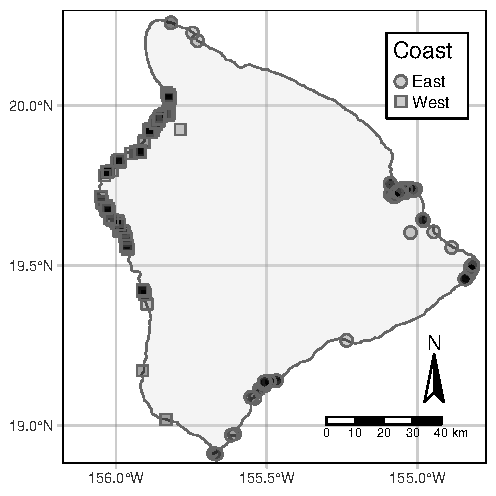
\includegraphics[width=\maxwidth]{figure/Figure-1} 
\end{knitrout}

\caption{Stranding locations and the division into eastern (windward) and western (leeward) sides of \Hawaii\ island. Coastline map courtesy of United States Geological Service (USGS) and \Hawaii\ Statewide GIS Program.}\label{fig:map}
\end{figure}

\begin{table}[tbp]
\caption{Raw counts and proportions of stranding cause from 1983--2022 for \Hawaii\ island, separated into east and west sides.
Fibropapillomatosis is abbreviated FP.
%The distribution is significantly different between sides (Chi-square test, $X_7=70$, $p < 10^{-10}$).
}\label{tab:cause}
\begin{knitrout}
\definecolor{shadecolor}{rgb}{0.969, 0.969, 0.969}\color{fgcolor}
\begin{tabular}{lrlrlrl}
\toprule
\multicolumn{1}{c}{ } & \multicolumn{2}{c}{East} & \multicolumn{2}{c}{West} & \multicolumn{2}{c}{Total} \\
\cmidrule(l{3pt}r{3pt}){2-3} \cmidrule(l{3pt}r{3pt}){4-5} \cmidrule(l{3pt}r{3pt}){6-7}
Cause & n & \% & n & \% & n & \%\\
\midrule
Boat impact & 9 & 2.4 & 16 & 4.3 & 25 & 3.3\\
FP & 53 & 14.0 & 1 & 0.3 & 54 & 7.2\\
Hook/line & 85 & 22.4 & 76 & 20.3 & 161 & 21.4\\
Human take & 19 & 5.0 & 14 & 3.7 & 33 & 4.4\\
Misc. & 5 & 1.3 & 23 & 6.1 & 28 & 3.7\\
Net & 7 & 1.8 & 9 & 2.4 & 16 & 2.1\\
Shark attack & 8 & 2.1 & 16 & 4.3 & 24 & 3.2\\
Unknown & 193 & 50.9 & 220 & 58.7 & 413 & 54.8\\
\bottomrule
\end{tabular}

\end{knitrout}
\end{table}

Of the 754 stranded turtles in the records, slightly over half had no known cause that could be determined (the ``unknown'' cause).
The most common known cause of stranding was hook-and-line fishing gear, accounting for about 1 in 5 strandings.
The distribution of causes is significantly different between the east and west coasts of the island (Chi-square test, $X_{7}= 69.5$, $p < 10^{-10}$), 
with the effect being driven most strongly by the FP and Miscellaneous categories (Table \ref{tab:cause}).

\subsection{Temporal trends}

The number of strandings on \Hawaii\ Island have fluctuated over the years but show an overall increase over time (Figure \ref{fig:sides}). 
Across both sides of the island, strandings were less frequent in winter, November--February, than in other months (Table \ref{tab:monthside}). 
The highest totals were observed between March and August.
Raw counts of hook-and-line fishing gear strandings have steadily increased over the years, and while strandings with FP as the chief cause of stranding have remained overall low, the number of FP-caused strandings was higher after 2000 (Figure \ref{fig:cause}).
The second most common known cause of stranding in west \Hawaii\ was miscellaneous, a category that includes a significant number of strandings associated with the 2011 T\={o}hoku tsunami, while in east \Hawaii\ FP is the second leading cause (Table \ref{tab:cause}, Figure \ref{fig:cause}).
%For both west and east \Hawaii, shark attack and boat impact strandings have increased over time (Figure8) (Figure 9). 
%A reduction in human take strandings over time is seen on east \Hawaii, and a peak of miscellaneous strandings is seen in 2011 on west \Hawaii\ (Figure 8) (Figure 9). 

\begin{figure}[tbp]

\centering
\begin{knitrout}
\definecolor{shadecolor}{rgb}{0.969, 0.969, 0.969}\color{fgcolor}
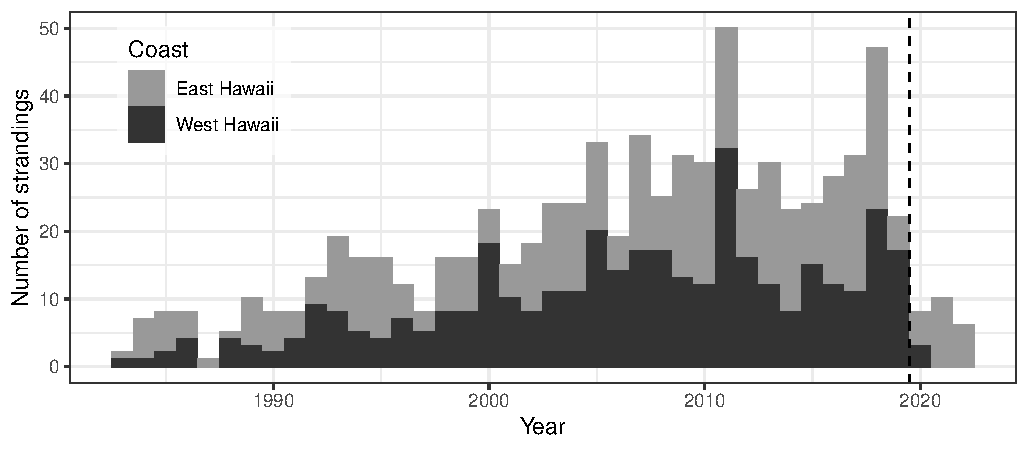
\includegraphics[width=\maxwidth]{figure/Figure-2} 
\end{knitrout}
\caption{Number of strandings from 1983--2022 for \Hawaii\ island, separated into east and west sides. Data for 2020 and beyond are incomplete due to COVID-19 disruptions to data collection.}
\label{fig:sides}
\end{figure}

\begin{table}[tbp]
\caption{Strandings in each month for \Hawaii\ island, separated into east and west sides.}\label{tab:monthside}
\begin{knitrout}
\definecolor{shadecolor}{rgb}{0.969, 0.969, 0.969}\color{fgcolor}
\begin{tabular}{lrrrrrrrrrrrrr}
\toprule
Coast & Jan & Feb & Mar & Apr & May & Jun & Jul & Aug & Sep & Oct & Nov & Dec & Total\\
\midrule
East & 29 & 31 & 32 & 38 & 33 & 42 & 37 & 30 & 25 & 33 & 25 & 24 & 379\\
West & 24 & 27 & 45 & 36 & 42 & 40 & 42 & 39 & 16 & 30 & 16 & 18 & 375\\
\addlinespace
Total & 53 & 58 & 77 & 74 & 75 & 82 & 79 & 69 & 41 & 63 & 41 & 42 & 754\\
\bottomrule
\end{tabular}

\end{knitrout}
\end{table}




\begin{figure}[tbp]
\centering
\begin{knitrout}
\definecolor{shadecolor}{rgb}{0.969, 0.969, 0.969}\color{fgcolor}
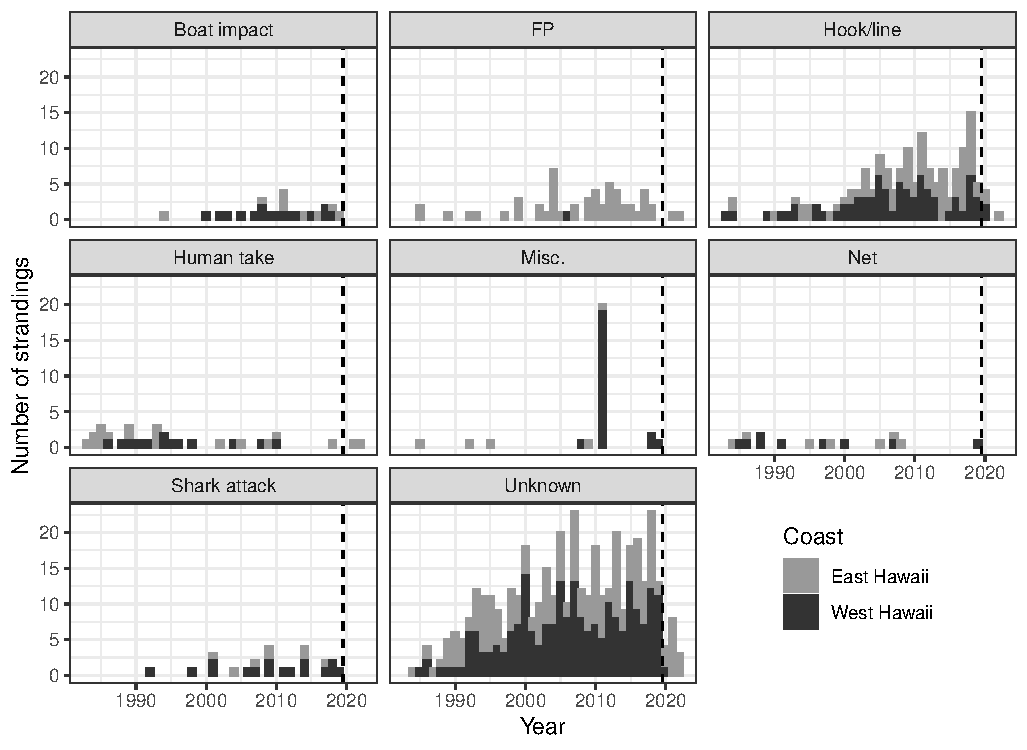
\includegraphics[width=\maxwidth]{figure/Figure-3} 
\end{knitrout}
\caption{Number of strandings from each cause, separated into east and west sides. Fibropapillomatosis is abbreviated FP. Data for 2020 and beyond are incomplete due to COVID-19 disruptions to data collection.}
\label{fig:cause}
\end{figure}









\begin{figure}[tbp]
\begin{knitrout}
\definecolor{shadecolor}{rgb}{0.969, 0.969, 0.969}\color{fgcolor}
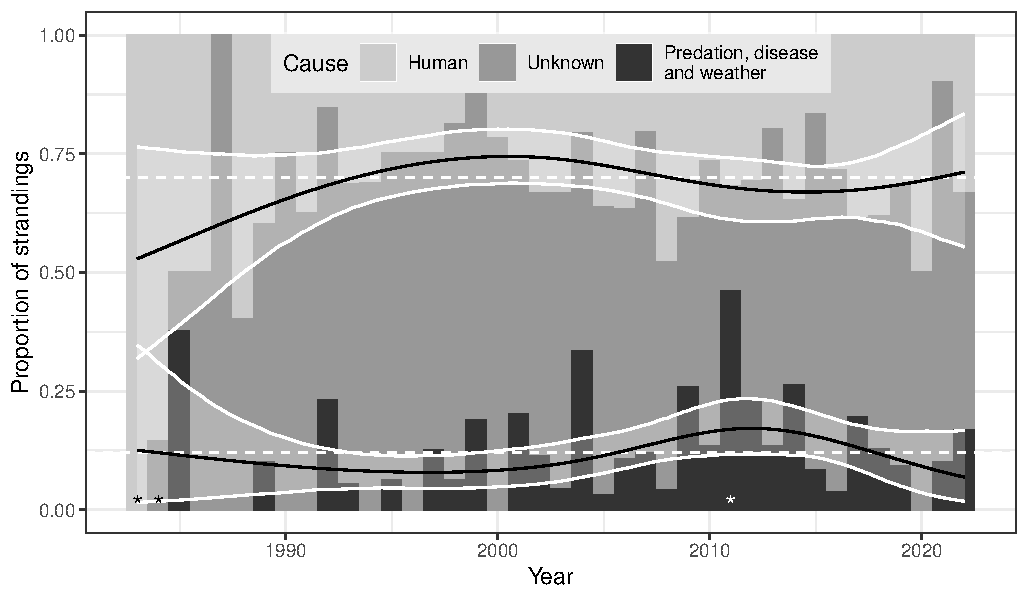
\includegraphics[width=\maxwidth]{figure/Figure-4} 
\end{knitrout}
\caption{A multinomial regression fit using natural splines with 3 degrees of freedom. 95\% confidence bands are constructed by bootstrapping. Records from years with asterisks (*) are excluded from the model. The dotted white lines correspond to a model with no dependence on year. 
%Akaike Information Criterion (AIC) of various models: zero degrees of freedom, $\text{AIC}=1300.9$; 1 degree, $\text{AIC}=1302.9$; 2 degrees, $\text{AIC}=1304.7$; 3 degrees, $\text{AIC}=1301.0$; 4 degrees, $\text{AIC}=1299.7$
}\label{fig:model}
\end{figure}


To investigate changes in the relative rates of stranding causes, multinomial log-linear models were fit using date of record as a predictor. 
To reduce the variance of the fitted model parameters, the causes as recorded were consolidated into 3 categories: Human caused (hook-and-line, boat impact, human take, and net); predation, disease and weather (shark attack, FP, and Misc.); and the original unknown category. 
The 2011 T\={o}hoku tsunami-related strandings, as well as the records prior to 1985 were excluded from the model fit.
The Akaike Information Criterion (AIC) is used to compare a series models of models using natural splines based on date of standing with increasing degrees of freedom.
The AIC increases going from a null model (AIC 1300.9) with no dependence on year
to a predictor function with 2 degrees of freedom (AIC 1304.7), 
and then slightly decreases again, so that a 4 degree of freedom model (AIC 1299.7)
has an AIC 1.2 smaller than the null model. 
Figure \ref{fig:model} displays a 3-degree of freedom model (AIC 1301),
with confidence bands constructed using the bootstrap.
The null model is represented by dotted white lines, and apparently fits within the confidence bands of the model that includes dependence on year. 
These results show a lack of evidence that the date of stranding provides significant information about the relative rates of stranding among the three consolidated cause categories.

\subsection{Size and gender}




Stranded turtles in the records ranged from 
19.8 cm to 
99 cm straight carapace length (SCL), with a mean of 
54.8 cm, across 
381 juveniles, 
88 subadults, and 
19 adults.
No carapace length measurement was recorded in 266 of the case reports.
Turtles stranding in east \Hawaii\ 
($\mu\pm\text{SE} = 58.7 
\pm 1$ cm SCL, $n=227$)
%\orig{($\mu\pm\text{SE}=58.8\pm0.78$ cm SCL, range 19.8--99 cm)} 
were significantly larger
(t-test, $t_{378}=6.29$,
$p=\ensuremath{9\times 10^{-10}}$)
%\orig{(t-test unequal variance, $t_{375}=6.32$, $p=7\times 10^{-10}$)}
than those in west \Hawaii\ 
($\mu\pm\text{SE} = 51.3 
\pm 0.6$ cm SCL, $n=261$)
%\orig{($\mu\pm\text{SE} = 51.3\pm0.51$ cm SCL, range 19.8--83 cm)}. 
Figure \ref{fig:length_cause} shows SCL distributions for each cause, and while the distribution of SCL is not independent of Cause (ANOVA, 
$F(7, 480)=3.41$, 
$p=0.0014$), 
the differences between the groups are small compared to the within-group variances.
The records contain 
154 female, 
145 male, and 
455 gender undetermined cases, also with marginally different distributions between side of the island (Chi-square, 
$X_{2}=6.4$,
$p=0.042$). 


\begin{figure}[tbp]
\begin{knitrout}
\definecolor{shadecolor}{rgb}{0.969, 0.969, 0.969}\color{fgcolor}
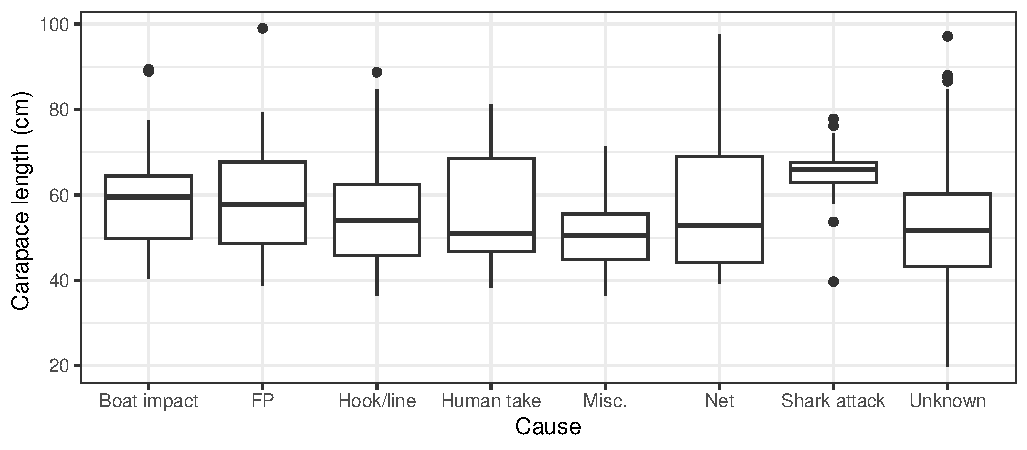
\includegraphics[width=\maxwidth]{figure/Figure-5} 
\end{knitrout}
\caption{Straight carapace length (SCL) was measured in 488 records, and and plotted for each stranding cause. Fibropapillomatosis is abbreviated FP. Boxplot outliers begin at 1.5 times the inter-quartile distance.}\label{fig:length_cause}
\end{figure}


\subsection{FP tumor presence/absence}

\begin{table}[tbp]
\caption{Fibropapillomatosis tumor presence in stranded turtles by side of \Hawaii\ island.
%Tumor distribution is unequal on the two sides of the island (Chi-square test, $X_2=198$, $p < 10^{-10}$).
}\label{tab:tumor_side}
\begin{knitrout}
\definecolor{shadecolor}{rgb}{0.969, 0.969, 0.969}\color{fgcolor}
\begin{tabular}{lrrr}
\toprule
\multicolumn{1}{c}{ } & \multicolumn{3}{c}{Tumor} \\
\cmidrule(l{3pt}r{3pt}){2-4}
Coast & Present & None & Not Recorded\\
\midrule
East & 141 & 143 & 95\\
West & 9 & 317 & 49\\
\addlinespace
Total & 150 & 460 & 144\\
\bottomrule
\end{tabular}

\end{knitrout}
\end{table}

As shown in Table \ref{tab:tumor_side}, 
460 records indicated the absence of FP tumors,
150 records presence of a tumor, and
144 records are missing this observation. 
Note that the presence of a FP tumor does not necessarily mean that the primary cause of stranding was recorded as FP. 
Tumor presence/absence is significantly associated with side of the island, with turtles stranding in east \Hawaii\ more likely to have tumors than those in west \Hawaii\ (Chi-square test, $X_2=197$, $p < 10^{-10}$).

\subsection{Stranding status}

\begin{table}[tbp]
\caption{Survival status of stranded turtles by cause. Fibropapillomatosis is abbreviated FP.
%Status is not independent of cause (Chi-square test, $X_{14}=102$, $p < 10^{-10})$.
}\label{tab:cause_status}
\begin{knitrout}
\definecolor{shadecolor}{rgb}{0.969, 0.969, 0.969}\color{fgcolor}
\begin{tabular}{lrrr}
\toprule
Cause & Alive & Dead & Not Recorded\\
\midrule
Boat impact & 12 & 13 & 0\\
FP & 38 & 16 & 0\\
Hook/line & 115 & 45 & 1\\
Human take & 6 & 27 & 0\\
Misc. & 23 & 5 & 0\\
Net & 8 & 8 & 0\\
Shark attack & 8 & 16 & 0\\
Unknown & 149 & 251 & 13\\
\addlinespace
Total & 359 & 381 & 14\\
\bottomrule
\end{tabular}

\end{knitrout}
\end{table}

\begin{table}[tbp]
\caption{Survival status of stranded turtles by month.}\label{tab:month_status}
\begin{knitrout}
\definecolor{shadecolor}{rgb}{0.969, 0.969, 0.969}\color{fgcolor}
\begin{tabular}{lrrr}
\toprule
Month & Alive & Dead & Not Recorded\\
\midrule
January & 31 & 20 & 2\\
February & 33 & 24 & 1\\
March & 49 & 28 & 0\\
April & 26 & 47 & 1\\
May & 25 & 45 & 5\\
June & 38 & 44 & 0\\
July & 35 & 43 & 1\\
August & 29 & 40 & 0\\
September & 17 & 23 & 1\\
October & 27 & 36 & 0\\
November & 24 & 17 & 0\\
December & 25 & 14 & 3\\
\bottomrule
\end{tabular}

\end{knitrout}
\end{table}




Of all the stranded turtles, 
359 stranded alive, 
381 stranded dead, and 
14 turtles had no stranding status reported.
Stranding status was found to be significantly associated with cause 
(Chi-square test, $X_{7} = 93$,
$p < 10^{-10}$).
More turtles stranded alive than dead because of FP, hook-and-line, and miscellaneous, while boat impact, human take, shark attack, and unknown were causes more likely to result in dead stranded turtles. 
Net fishing gear strandings showed equal numbers of turtles that stranded alive and dead (Table \ref{tab:cause_status}).
More turtles stranded alive than dead in the months of November--March, while more turtles stranded dead than alive in the months of April--October (Table \ref{tab:month_status}).
Stranding status was also found to be significantly associated with stranding location (Chi-square test,
$X_{1} = 21.5$, 
$p = \ensuremath{3.5\times 10^{-6}}$).
West \Hawaii\ had
146 turtles strand alive and
221 strand dead, 
while east \Hawaii\ had 
213 turtles strand alive and
160 strand dead. 

%%%%%%%%%%%%%%%
%%% DISCUSSION
%%%%%%%%%%%%%%%

\section{Discussion}

Seven hundred fifty-four green turtles were recorded stranded on \Hawaii\ Island in the period 1983-2022, which represents an unknown fraction of total strandings on Hawaiian shores in that time. 
Stranding programs rely on reports from the public, and are therefore dependent on the density of human activity at the shoreline as well as public knowledge of the reporting procedures.
However, if a location is regularly accessed by more than a few people, a stranding is likely to be reported, and it is reasonable to believe that this will happen independent of the variables observed in these records.
%However, strandings that are reported are probably an accurate reflection of the distribution, demographics, and causes of \Hawaii\ Island strandings. 

Strandings on \Hawaii\ Island showed an overall increase in rate between 1983 and 2022. Green turtle strandings have also increased on the other main Hawaiian Islands since 1982 \citep{chaloupka2008cause}.
One important reason for this increase is a positive one: Green turtle populations in the Hawaiian Islands have recovered significantly since their 1974 protection by the State of \Hawaii\ under Regulation 36 and their 1978 protection under the Endangered Species Act \citep{balazs2004thirty, bennett2008book}.
The increase in population size will directly lead to additional observed stranding events, even if the risk to an individual turtle remains constant over time \citep{boulon2000trends}. 
Additionally, the human population increase on \Hawaii\ Island and the rise in numbers of visitors at the shoreline increase the chance of encountering and reporting a stranding. 
In general, the locations of strandings shown in Figure \ref{fig:map} reflect beaches and other shoreline areas with easy public access.
Increased public awareness of strandings and response programs and the greater use of cell phones and the internet probably have led to more reporting over time.
However, the increase in reported strandings appears to slow in the early 2000s (Figure \ref{fig:sides}), stabilizing at approximately 25--30 per year.
This trend was also noticed in studies covering the other main Hawaiian Islands \citep{chaloupka2008cause}. 

There are two years post 2005 which show an unusually large number of Green turtle strandings: 2011 and 2018. The peak in 2011 is associated with the March 2011 magnitude 9.0 T\={o}hoku earthquake off the coast of Japan and the subsequent tsunami, large waves, and hazardous currents that it caused around \Hawaii\ Island, and particularly its western shoreline \citep{cheung2013surges}. 
The waves and currents associated with tsunamis bring marine life onshore with them and can wash turtles inland. 
Two hawksbill turtles were reported stranded in \Hawaii\ as a result of the 2011 earthquake \citep{brunson2022three}, and a 2009 tsunami in Samoa similarly led to 52 turtles stranding on land \citep{bell2011marine}. 
The apparent downward trend of strandings after 2018 is probably not because fewer turtles stranded, but is rather due to human behavioral changes caused by the COVID-19 pandemic.
Throughout the pandemic, people in general spent much less time in public locations, and for some periods, \Hawaii\ County and State beach parks were closed for recreational use by executive decree \citep{emergencyNo2, emergencyFifth}.
Similarly, tourism to the island and state was heavily restricted.
All of these factors lead to a sharp drop in the number of people visiting \Hawaii\ Island coasts, and subsequent reports of strandings. 

The highest rates of green turtle strandings occurred during the Hawaiian spring and summer months, from March--August.
This is similar to the findings on \Oahu\ where green turtle strandings were highest from March--June \citep{chaloupka2008cause}, and for adult hawksbills in the Hawaiian Archipelago where strandings were highest from June--September \citep{brunson2022three}. 
Similarly, strandings of loggerhead, green, and leatherback turtles in Brazil were highest during the austral spring and summer seasons \citep{monteiro2016long}. 
Strandings on \Hawaii\ Island were lowest during the months of September, November, and December, but a secondary peak in the month of October was seen.
This same peak was observed in the 2022 green turtle strandings on Maui \citep{cutt2023impact} and
\Oahu\ showed a similar secondary peak of strandings in September \citep{chaloupka2008cause}. 
This trend of strandings seen in the Hawaiian Islands may indicate seasonal abundance of turtles, seasonal activity of humans, or seasonality of shoreline surf, currents, and winds \citep{chaloupka2008cause}.

Hook-and-line fishing gear was the most common known cause of stranding of green turtles on \Hawaii\ Island as a whole.
Fishing gear strandings show a similar qualitative pattern to the overall time series (Figure \ref{fig:cause}), increasing from 1983 to the mid 2000s and then apparently leveling off. 
\cite{chaloupka2008cause} found a similar increase of hook-and-line fishing gear strandings since 1982.
It is difficult to untangle the effects of the increased population of Hawaiian green turtles from the risk of hazard from fishing activity and gear, as both factors directly affect the rate of strandings observed.

Hawaiian green turtles are frequently reported with hooks intact and line entangled around their flippers and body. 
These interactions are often a result of lost and/or discarded fishing gear or fishers cutting the line when accidental hooking occurred, which illustrates the need for stronger management and preventatives \citep{nitta1993review}. 
Hook-and-line fishing gear strandings were also prevalent on \Oahu, Maui, and Kauai, making up the second most common cause of stranding of green turtles \citep{chaloupka2008cause}.
Similar to the findings of the present study, fishing gear was the foremost cause of stranding for green turtles on Maui in 2022, with 81\% of the total strandings showing interactions \citep{cutt2023impact}.

However, the number of hook-and-line strandings may be even greater than estimated. 
\cite{work2015causes} performed necropsies (postmortem autopsies) on stranded turtles throughout the Pacific and found that 48\% of foreign body ingestion cases (mostly all associated with fishing gear) showed no external sign of fishing line interactions.
Green turtle strandings resulting from interactions with fishing gear are prevalent around the world, including the U.S. Virgin Islands \citep{boulon2000trends}, Brazil \citep{guimares2021distribution}, Taiwan \citep{cheng2019twenty}, and Greece \citep{panagopoulos2003stranding}. 
Fibropapillomatosis was the second most common cause of stranding in this study, whereas \cite{chaloupka2008cause} found FP to be the main cause of stranding in green turtles in \Oahu, Maui, and Kauai. 

The relative rates of strandings by cause over time is of particular interest for managers and conservationists because it can indicate particular sources of danger to turtle populations. 
The overall rate of observation depends on population size and human reporting behavior in a complex way that is difficult to disentangle, but by looking at the distribution of causes over time we may be able to identify structural changes in the cause of strandings.
While the record collection process kept eight categories of cause, for modelling purposes we reduced these to 3 broad categories: direct intentional and accidental human causes, such as boat impacts and fishing and hunting related injuries; natural events, predation, and disease; and unknown causes. 

The distribution of these three consolidated causes has been relatively stable since the early 1990s (Figure \ref{fig:model}), providing unconvincing evidence of any major shifts between the relative risks between direct human causes and the other categories.
One way of interpreting this result is that the increased numbers of strandings over time can be explained entirely by the growth in turtle populations and increases in reporting by the public. 
While keeping the proportion of human-caused strandings constant over time may be regarded as a minor conservation success story, given the significant growth in human population and coastal activity over the same time period, humans remain a significant source of danger to turtles.
There remains much room for improvement, in particular with regards to hook-and-line injuries.


The current study found that different sides of \Hawaii\ Island had different distributions of stranding cause. West \Hawaii\ Island had a higher proportion of shark attack and boat impact strandings, while east \Hawaii\ had more FP and human take strandings.
Increased shark attack strandings on west \Hawaii\ may be because of the larger population of tiger sharks found along the west coast \citep{meyer2009long}. 
Tiger sharks are well-known predators of sea turtles, and green turtles are found regularly in their stomach contents \citep{witzell1987selective, lowe1996ontogenetic}. 
West \Hawaii\ also has a large tourism industry, with many snorkel, diving, and manta ray and marine mammal watching tours operating in the same coastal waters that green turtles occupy. 
These tours, as well as commercial vessels, frequent the many shallow bays located in west \Hawaii\ that are important foraging habitats for green turtles. 
Increased boat presence accompanied with high vessel speeds, varying water depth, and times of poor visibility can all factor into a higher proportion of boat impact strandings on the west side of the island \citep{fuentes2021conservation}.

The majority of green turtles that stranded on \Hawaii\ Island were juveniles. Similarly, juveniles predominated the stranded green and hawksbill turtles throughout the Hawaiian Islands \citep{chaloupka2008cause, brunson2022three}.
Juvenile green turtles were also the most common size class stranded in New Caledonia \citep{read2023twenty}, Australia \citep{flint2015trends}, and Brazil \citep{monteiro2016long}. 
The high proportion of juveniles stranding may be a result of increased nesting populations at French Frigate Shoals leading to an increase in juveniles moving from nesting to foraging areas \citep{balazs2004thirty}.
Juvenile turtles may be more immunologically na\"{i}ve and susceptible to environmental stressors that could contribute to stranding \citep{flint2015trends}. 

Larger turtles stranded on east \Hawaii\ Island than on west \Hawaii, despite the fact that stranded turtles with the highest SCL values were the result of shark attacks.
\cite{bornatowski2012shark} found that the probability that a green turtle in Brazil stranded with a shark bite increased with size, and \cite{chaloupka2008cause} reported the same trend for green turtles in the main Hawaiian Islands.
Smaller green turtles are also frequently attacked by sharks, but may be completely consumed and thus do not wash ashore after such event.
A spatial trend in size-classes was also reported by \cite{chaloupka2008cause}: larger turtles stranded on Maui and Kauai than on \Oahu.

There was no gender-bias of stranded green turtles on \Hawaii\ Island: male and female strandings occurred with a 1:1.06 ratio.
The lack of a gender-bias for green turtles was also shown in the main Hawaiian Islands \citep{work2004retrospective, chaloupka2008cause}. 
The present and prior studies are consistent with the 1:1 sex ratio of Hawaiian green turtles found by \cite{wibbels1993sex}. Unlike in the Hawaiian Islands, many green turtle populations around the world appear to have more females than males \citep{flint2010health, cheng2019twenty, read2023twenty}. 
Clutches of sea turtles are sensitive to temperature change, and an increase in the temperature during incubation can drastically change sex ratios of nests, leading to clutches of all females. 
As temperatures continue to rise as a result of climate change, the Hawaiian population of green turtles may eventually see the same skew seen in other locations around the world \citep{hawkes2009climate}.

More than 60\% of the stranded turtles on \Hawaii\ Island had no tumors indicative of FP, although this is likely an overestimate of the true value, as not every turtle in this study underwent a necropsy that could reveal the presence of internal tumors that would otherwise go unreported.
However, the overall reduction of FP prevalence has been documented previously in Hawaiian green turtles.
Twenty-one of 66 turtles observed with tumors in one summer were then seen later with no tumors \citep{bennett2000photographic}.
The low population of turtles with FP on \Hawaii\ Island is consistent with the 2022 stranding report for green turtles on Maui, in which only one case of FP was reported \citep{cutt2023impact}. 

Turtles were more likely to have FP on east \Hawaii, whereas FP was very rare on green turtles that stranded on west \Hawaii. 
The west (Kona) coast of \Hawaii\ Island had no diagnosed cases of FP for many of the years that FP was prevalent in the other Hawaiian Islands \citep{balazs1991current, aguirre2000blood, work2001immune}. 
In Florida, turtles with tumors are more likely to become entangled in fishing line, thus the higher percentage of hook-and-line strandings that occurred on east \Hawaii\ may be a result of higher FP presence \citep{foley2005fibropapillomatosis}. 
However, \cite{chaloupka2008cause} found no correlation between FP and fishing gear strandings in the other main Hawaiian Islands. 
Similar to the spatial variation in FP infection on \Hawaii\ Island, FP was more often found in \Oahu\ and Maui than on Kauai \citep{chaloupka2008cause}. 
Green turtles that stranded on the western (Gulf) coast of Florida (51.9\%) were more likely to have tumors than turtles that stranded on the eastern (Atlantic) coast (11.9\%) \citep{foley2005fibropapillomatosis}. 
In Australia, FP varied in prevalence from 0 to 11.6\% at 15 sites all along the Queensland coast \citep{jones2022spatial}. 

A variety of factors have been hypothesized for the varying prevalence of FP in different locations and may be the reason for the contrasting FP abundance on west and east \Hawaii\ Island.
For example, FP in Florida was greatest in areas with the greatest habitat degradation and pollution, most shallow water areas, and lowest wave-energy level, indicating that one or more of these conditions may affect FP \citep{foley2005fibropapillomatosis}.
In Brazil, highly urbanized areas have a higher FP prevalence than lightly urbanized areas \citep{bastos2022coastal}. 
Additionally, FP may be related to water temperature, with higher water temperatures correlated with greater FP prevalence \citep{manes2022occurrence}. 
An important factor that could contribute to the absence of FP on west \Hawaii\ is the precipitation pattern on the leeward side of the island.
The windward (east) side, experiences abundant, consistent rainfall and has large rivers and many streams \citep{juvik1998atlas}. 
Heavy rain may bring more land-based pollutants to rivers, and the discharge from these rivers located in urbanized areas may disrupt the immune system of green turtles, making them more susceptible to FP \citep{manes2022occurrence}. 
Despite the low rainfall and lack of flowing surface water in west \Hawaii, coastal waters can experience nutrient pollution via submarine groundwater discharge, which could impact green turtle health \citep{abaya2018spatial, abaya2018multi, panelo2022spatial}.
	
The relatively even distribution of turtles that stranded alive (359) versus dead 381 on \Hawaii\ Island in the present study is markedly different from the findings of \cite{chaloupka2008cause}, where on \Oahu, Maui, and Kauai approximately 75\% of green turtles stranded dead. 
In the present study, stranding status was found to vary temporally, by cause, and spatially. 
Green turtles were more likely to strand alive in the winter months (November--March), and dead in the summer months (April--October).
Additionally, more turtles stranded dead than alive because of boat impacts, human take, and shark attacks, similar to other Hawaiian Islands, where boat impact and shark attack were the hazards most likely to result in a dead turtle \citep{chaloupka2008cause}.
Shark attacks often cause the loss of appendages and boat impacts usually cause damage to the head, appendages, and/or the carapace, all serious injuries that lead to significant mortality.
The present study found that turtles that stranded as a result of FP were more likely to strand alive than dead, unlike findings of \cite{chaloupka2008cause}. 
More turtles stranded dead than alive on west \Hawaii and more turtles stranded alive than dead on east \Hawaii, probably because shark attacks and boat impacts are more common on west \Hawaii, while FP is reported almost exclusively on eastern shores. 
\cite{chaloupka2008cause} found that the probability of mortality in a stranding decreased with turtle size, and this pattern is also observed in this data across the two sides of \Hawaii\ Island.

Despite the large percentage of unknown causes of stranding, this long-term data set provides important information on \Hawaii\ Island green turtle strandings.
Continued monitoring of turtle strandings and careful data collection on stranded individuals is critical to the conservation of green turtles.

The considerable contribution of hook-and-line fishing gear to strandings highlights the continuing need for additional mitigation efforts, such as barbless hooks and effective line removal techniques (\url{https://dlnr.hawaii.gov/dobor/marineanimalhotline/}), focused on green turtle interactions with fisheries.

\section{Compliance with Ethical Standards}

The authors declare that no funds, grants, or other support were received to assist in the preparation of this manuscript.
The authors have no relevant financial or non-financial interests to disclose.

Study conception and design by Skylar Dentlinger and Karla J. McDermid. 
Initial analysis and first draft prepared by Skylar Dentlinger. 
Follow-up analyses and modeling by Grady Weyenberg. 
All authors contributed to editing and revision of the manuscript and have read and approved the finalized version.

This is an observational study compiled from publicly available records. 
No ethical approval is required.
All data analyzed during this study are included in this published article and its supplementary information files.


\section{Acknowledgements}
We would like to thank the following individuals, agencies, and organizations that contributed to data collection and/or mentorship:
Summer Martin, 
Brittany Clemans, 
Jen Sims, 
Megan Lamson, 
Rebecca Ostertag, 
NOAA Marine Turtle Biology \& Assessment Program,
University of  \Hawaii\ at Hilo Marine Option Program Sea Turtle Stranding Response Team,
\Hawaii\ Preparatory Academy Sea Turtle Research Program,
and the State of \Hawaii\ Department of Land and Natural Resources.

\bibliography{turtles}

\end{document}
